
\newcommand{\subeventtype}{Sub-Event-Type }
\newcommand{\tcp}{TCP/IP }
\newcommand{\dataconverterplugin}{Data-Converter-Plugin }
\newcommand{\eventid}{Event-ID }
\newcommand{\cpp}{C++ }
\newcommand{\producer}{producer }
\newcommand{\eventtype}{Event-Type }
\newcommand{\event}{Event }
\newcommand{\eventheader}{Event-Header }
\newcommand{\timestamp}{Time-Stamp }
\newcommand{\rawdata}{Raw-Data }
\newcommand{\datablock}{Data-Block }
\newcommand{\da}{Data-Acquisition }
\newcommand{\dc}{Data-Collector }
\newcommand{\onlinemon}{Online-Monitor }
\newcommand{\hitmaps}{Hit-Maps }
\newcommand{\corplots}{Correlation-Plots }
\newcommand{\offlineana}{Offline-Analysis }
\newcommand{\filewriter}{File-Writer }
\newcommand{\rc}{Run-Control }
\newcommand{\testrc}{TestRunControl }
\newcommand{\logcollector}{Log-Collector }


Pasting  from other another section:

\eudaq serves as a tool set and an integration layer for the user DAQ system(s), providing the communication protocols for them to participate in a common DAQ. 


The functionality is contains three separated areas. 

- Data-Acquisition
- Data-Quality-Monitoring 
- Data Conversion (LCIO)

\subsection{Data-Acquisition}


\eudaq is a modular cross platform data Acquisition System designed in the context of the \eudet project. 
It consist of completely independent modules such as \rc, \logcollector, \dc and \producer. 
The communication between individual modules is done via \tcp therefore it is possible to run each module on a separate PC. 


\begin{figure}[tb]
	\center
	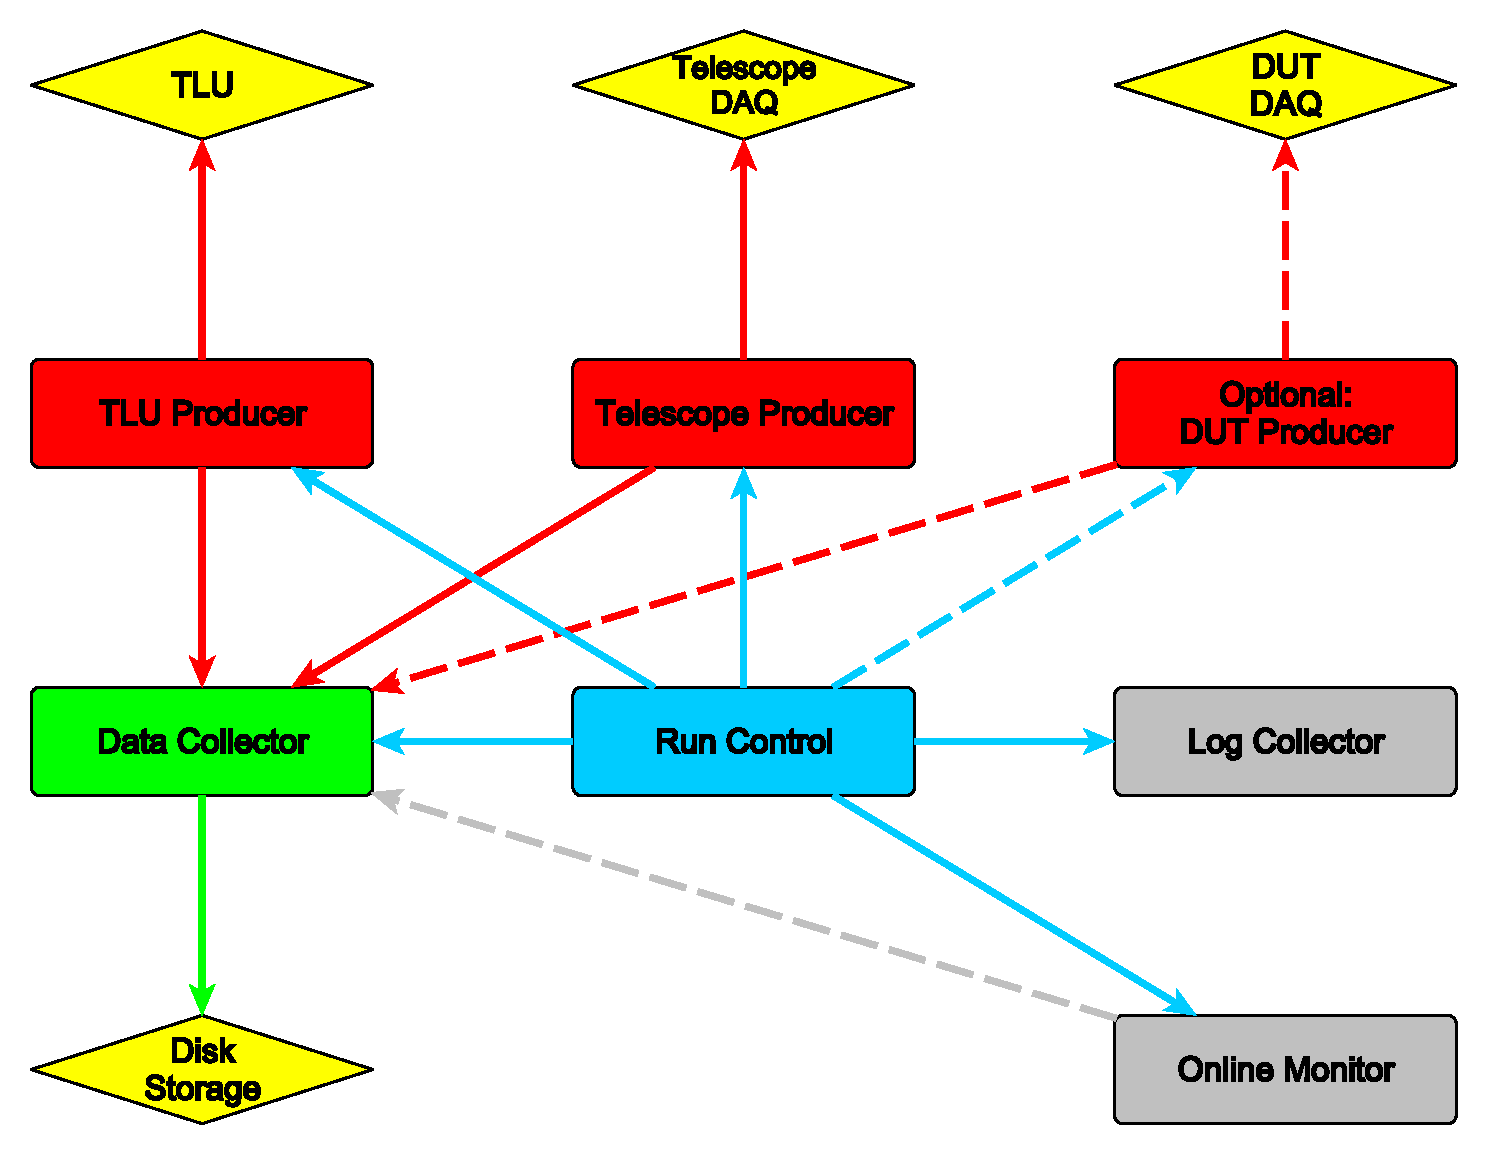
\includegraphics[width=.55\textwidth]{figures/eudaq}
	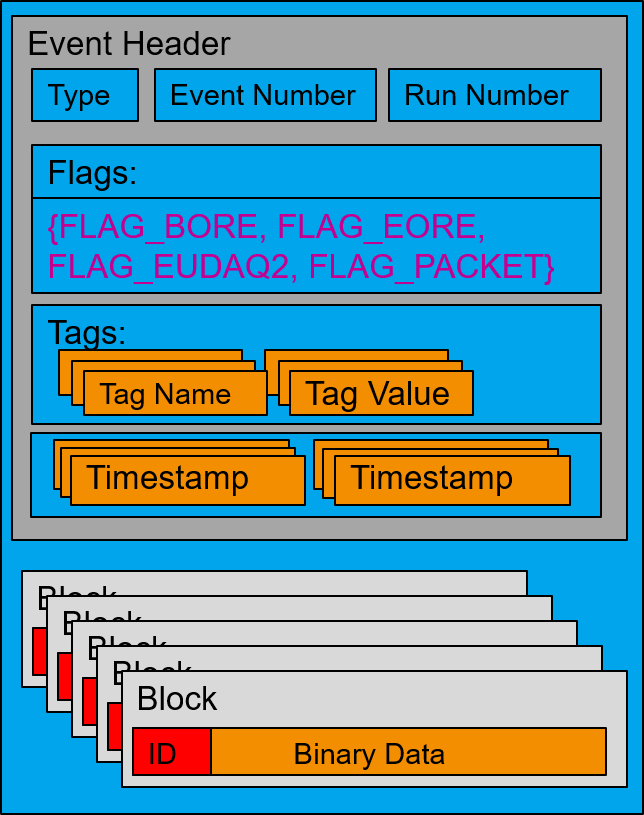
\includegraphics[width=.38\textwidth]{figures/rawdataevent.png}
	\caption[DAQ_System]{(A) Hardware and software layout of the DAQ system. (B) \rawdataevent}
	\label{fig:todo}
\end{figure}

% \begin{figure}[tb]
% 	\center
% 	
% 	\caption[DAQ_System]{\rawdataevent}
% 	\label{fig:todo}
% \end{figure}


% RunControl
The \rc is the central point for human interactions. 
From it the producer are configured, started, stopped and terminated. 
Currently there are two implementation of the \rc one command line version called \testrc and one GUI version Called euRun. 
Both have the about same functionality. The \testrc is scriptable which allows the users to run fully automated. 

% Log collector 
The \logcollector receives all status/error messages that are produced by any of the \producer. 
It has the possibility to filter for different warning levels. 

%data Collector 
The \dc has a direct connection do all the producer. 
\eudaq 1.x is an event based DAQ system, therefore the \dc expects that all \producer send one \event per trigger that they have received from the TLU. And that all events from different \producer share a common trigger number by which they get merged into one container event called Detector-Event. 
The \dc has the possibility to do some basic sanity checks on the events like event number mismatch. The \dc is able to handle unknown event types, therefore it is possible to run a new \producer with an old \dc. It is not necessary to recompile the \dc to tun it with a new \producer. 

%producer 
The \producer handles the communication between the \eudaq framework and the user DAQ system. 
The user has to write its own \producer class which inherits from the abstract class producer. 
This base class encapsulates the \tcp communication. The \producer has three states: unconfigured, configured and running. The \producer packs the data readout by the users DAQ system in an \eudaq \event and sends it over \tcp to the \dc. 

%data converter plugin 
The \dataconverterplugin is used to convert the \rawdata send by the \producer to hit information. 


%config files 
The configuration file is a plain text file which contains a section for each producer. 
Each sections contains tag-value pairs for the configuration of the producer. 
Sections for producer that are currently not connected are ignored. 

% Event format 
 The idea behind the \event class in \eudaq is that the it is used as data container with only a very limited set of functionality. All the advanced functionality is part of the \dataconverterplugin. The basic \event type that is used for user's data is the \rawdataevent. Its structure is shown in figure ??. It consist of an \eventheader and a \datablock. 

% Event header 
In the \eventheader the \eventtype is stored. The \eventtype is used to determine which \dataconverterplugin to call for the this \event. The \eventype consist of two part the \eventid and the \subeventtype. The \eventid indicates the \cpp class. The \subeventtype is used to uniquely identify the \event. It is set in the \producer by the user. In the \eventheader is also a field to store flags to indicate some specialty of this \event. This can for example be the information if it is a Begin-Of-Run-Event (BORE) or End-Of-Run-Event (EOFE). In addition the \eventheader can store a \timestamp. 
 
%event body
The \datablock contains the \rawdata from the detector. The serialization/de-serialization is the users responsibility. \eudaq provides some functionality for this but the user is free to use its own more elevated mechanisms. 
 

\subsection{Data-Quality-Monitoring}

\eudaq has basic functionality to check during the run the quality of the data. One is that already the \dc checks if the data arrive in the right order and checks for possible mismatches. The second more elevated mechanisms is the \onlinemon. Which collects during run the data from the \dc and produces \hitmaps and \corrplots. In addition this  plots can also be saved in a ROOT file. To make this work the \onlinemon needs to have the \dataconverterplugin for all devices in use. The \onlinemon can also run offline using files on disk.


\subsection{Data-Conversion}
For the \offlineana it is necessary to convert the data from the RAW format \eudaq uses internally to a format that is use by the reconstruction software the user uses for their analysis. \eudaq gives the possibility to implement user specific \filewriter. Among many others the \filewriter which are most important at the moment are the following three 

- Plain text
- ROOT TTRee 
- LCIO 





